
% Szkielet dla pracy inżynierskiej pisanej w języku polskim.

\documentclass[polish,master,a4paper,oneside]{ppfcmthesis}


\usepackage[utf8]{inputenc}
\usepackage[OT4]{fontenc}
\usepackage{graphicx}
\usepackage{float}


% Authors of the thesis here. Separate them with \and
\author{%
   Wojciech Kopeć \album{101675} \and
} 
\title{Imitation Learning}                   % Note how we protect the final title phrase from breaking
\ppsupervisor{dr~inż.~Krzysztof Dembczyński} % Your supervisor comes here.
\ppyear{2017}                                         % Year of final submission (not graduation!)


\begin{document}

% Front matter starts here
\frontmatter\pagestyle{empty}%
\maketitle\cleardoublepage%

% Blank info page for "karta dyplomowa"
\thispagestyle{empty}\vspace*{\fill}%
\begin{center}Tutaj przychodzi karta pracy dyplomowej;\\oryginał wstawiamy do wersji dla archiwum PP, w pozostałych kopiach wstawiamy ksero.\end{center}%
\vfill\cleardoublepage%

% Table of contents.
\pagenumbering{Roman}\pagestyle{ppfcmthesis}%
\tableofcontents* \cleardoublepage%

% Main content of your thesis starts here.
\mainmatter%
W poniższym rozdziale przedstawione są badane i zaimplementowane w pracy podejścia.

Każde z rozwiązań działa w ramach wspólnego szkieletu, bazującego na przykładowych rozwiązaniach towarzyszących środowisku VizDoom. Dzięki temu możliwe jest bezpośrednie porównanie zachowania różnych podejść przy zmianie tylko kluczowych algorytmów przy zachowaniu niezmienności pozostałych czynników.

\chapter{Niepewność}
\section{Niepewność - uproszczony eksperyment}
W celu porównania skuteczności Bootstrapa i Dropout w ocenianiu niepewności wyników sieci przeprowadzono prostszy eksperyment na lepiej znanych i kontrolowanych danych. Do eksperymentu wykorzystano zbiór MNIST [REF] zawierający odręcznie pisane cyfry. MNIST jest często używany jako przykładowy zbiór danych, służący do przystępnej prezentacji i porównań metod uczenia maszynowego. Najczęściej wykorzystywany jest w kontekscie klasyfikacji, jednak traktowanie wartości liczbowych cyfr jako etykiet (w przeciwieństwie do stosowanego w klasyfikacji one-hot encoding [REF]) w oczywisty sposób prezentuje problem regresji.    

\subsection{Eksperyment}
W ramach eksperymentów uczono sieć neuronową na niezbalansowanych zbiorach danych bazującym na MNIST. Dobrane dystrybucje przykładów o konkretnych etykietach w danych uczących mają pokazać, jak poszczególne techniki zachowują się wobec zupełnie nieznanych danych i mało znanych danych. Zbiór danych mnist składa się z 60 tysięcy przykładów uczących i 10 tysięcy przykładów treningowych. KAżdy obrazek przedstawia jedną czarno-białą cyfrę i ma rozmiar 28x28 pikseli. W eksperymencie etykiety zostały przeprasformowane liniowo z przedziału $[0,9]$ do $[-0.5,0.5]$.

Pierwszy, prostszy, eksperyment posłużył również do znalezienia optymalnych parametrów obu metod. Drugi eksperyment został przeprowadzony z wykorzystaniem znalezionych wcześniej parametrów. Każdy z eksperymentów został powtórzony 10 razy.

\subsubsection{Rozpoznawanie nieznanych danych}
Zachowanie wobec nieznanych danych zbadano ucząc sięć neuronową wyłącznie na przykładach parzystych cyfr. W wynikowej klasyfikacji stopień niepewności zwracanych wyników powinien być znacznie wyższy dla cyfr nieparzystych niż parzystych.


\subsubsection{Ocena stopnia pewności wyników}
Zachowanie wobec mało znanych danych zbadano ucząc sieć neuronową na niezbalansowanym zbiorze danych. Przykłady trafiały do zbioru uczącego z prawdopodobieństwem proporcjonalnym do przedstawianej cyfry, przykładowo 0 z prawdopodobieństwem $p=0$, 5 z prawdopodobieństwem $p=0.5$ i 9 z prawdopodobieństwem $p=0.9$. W wynikowej klasyfikacji stopień niepewności zwracanych wyników powinien być zależny od prawdopodobieństwa trafienia do zbioru danej etykiety.

\subsection{Implementacja bazowa}
Bazą dla implementacji użytych w eksperymencie był przykład klasyfikacji zbioru MNIST za pomocą konwolucyjnych sieci neuronowych udostępniony z biblioteką Tensorflow. Użyta w przykłądzie sieć składa się z dwóch warstw konwolucyjnych i dwóch warstw w pełni połączonych.

W ramach obu eksperymentów uczenie trwa 1 milion iteracji, a wielkość batcha wynosi 128. Prędkość uczenia wynosi $0.005$, przy czym dla Bootstrapu ta wartość jest normalizowana przez średnią liczbę użyć każdego przykładu.

\subsection{Miary jakości}
Kluczowe dla określenia jakości obu metod jest zdefiniowanie miary jakości wyników. Docelowo przyjęta miara powinna dobrze oddawać przydatność do oceny stanu przez agenta DQN.

Za miarę niepewności przyjęto rozstęp międzykwartylowy próbek uzyskanych z sieci. O wyborze rozstępu międzykwartylowego zdecydowała większe od odchylenia standardowego odporność na skrajne wartości. Oprócz rozstępu międzykwartylowego sprawdzono eksperymentalnie również wariancję (która dawała nieznacznie gorsze wyniki) i różnicę między skrajnymi wartościami (zależność od skrajnych wartości uczyniła tą miarę bardzo niestabilną i mało skuteczną).

\[ unc = q(75) -q(25)\]

\subsubsection{Rozpoznawanie nieznanych danych}
Liczba znanych i nieznanych etykiet w zbiorze tekstowym jest równa, dlatego za miarę jakości rozdziału danych znanych i nieznanych przyjęto stosunek sumy średnich niepewności dla kolejnych nieznanych etykiet do sumy niepewności dla kolejnych znanych etykiet. Wartości bliskie 1 oznaczają brak rozdziału danych. W eskperymentach wynikowe miary nie przekraczały wartości 2.
\[ quality_{ND} = \frac{\sum_{l \in \{unknown\}} \overline{unc_{l}}}{\sum_{l \in \{known\}} \overline{unc_{l}}}\]

\subsubsection{Ocena stopnia pewności wyników }
Niepewność powinna być odwrotnie proporcjonalna do trafności klasyfikacji, dlatego za miarę jakości oceny niepewności wyników przyjęto wartość absolutną współczynnika korelacji pomiędzy średnią niepewnością a średnią trafnością klasyfikacji dla kolejnych etykiet. Użyta we właściwym eksperymencie współczynnik regresji jest liczony dla etykiet od 1 do 9, ponieważ zerowa trafność dla etykiety 0 jest wspólna dla obu metod i wyraźnie zaburza wyraźnie liniową zależność reszty.

\[ quality_{OP} = |r_{unc\ acc}|\]

\subsection{Dropout - konfiguracja}
Dropout został dodany pomiędzy ostatnią warstwą konwolucyjną sieci a pierwszą w pełni połączoną oraz pomiędzy obiema w pełni połączonymi warstwami.
Parametry modelu to prawdopodobieństwo zachowania neuronu w czasie treningu $p_{train}$, prawdopodobieństwo zachowania neuronu w czasie testu $p_{test}$ i liczbę odpytań sieci $n$ przy określaniu niepewności. W eksperymentach sprawdzano wartości $p_{train} \in \{0.25, 0.5, 0.75, 1\}$, $p_{test} \in \{0.25, 0.5, 0.751\}$ i $n \in \{10, 30, 50, 100\}$.

Zastosowana \href{https://link.do.pliku}{implementacja z wykorzystaniem Tensorflow} wymaga każdorazowego przeliczenia wszystkich wartości przy każdym pojedyńczym odpytaniu.

\subsection{Bootstrap - konfiguracja}
Bootstrapowana sieć ma wspólne warstwy konwolucyjne. Z warstw konwolucyjnych wychodzi $n$ niezależnych "głów", skłądających się z dwóch warstwy w pełni połączone wykorzystanych w przykładzie bazowym. Parametry modelu to liczba "głów" $n$ i prawdopodobieństwo uwzględnienia krotki danych przez głowę $p_{incl}$.  W eksperymentach sprawdzano wartości $n \in  \{5,7,10\}$ i $p_{incl}\in\{0.25, 0.5, 0.75, 1\}$.

Zastosowana \href{https://link.do.pliku}{implementacja z wykorzystaniem Tensorflow} decyduje o uwzględnianiu przez poszczególne głowy dla pełnych batchy danych, a nie dla pojedynczych krotek. Przy odpytywaniu kilku głów o ten sam przykład przeliczenie warstw konwolucyjnych następuje tylko jednokrotnie.



\subsection{Niepewność - wyniki eksperymentu z nieznanymi danymi}

Na wykresach \ref{fig:b_ratio_mean}, \ref{fig:d_ratio_mean}, \ref{fig:d_ratio_mean2}, \ref{fig:d_ratio_var2}, \ref{fig:b_ratio_var}, \ref{fig:d_ratio_var} przedstawiono średnie i odchylenia standardowe miary jakości $quality_{ND}$ uzyskane dla poszczególnych konfiguracji eksperymentów. Największa wartość $quality_{ND}$ uzyskana za pomocą Bootstrapa (1.565 dla 5 głów i prawdopodobieństwa 1) jest wyższa niż największa wartość uzyskana za pomocą Dropoutu (1.424 dla 30 wywołań i prawdopodobieństw dropoutu = 0.75). Wyniki bootstrapa dla tych parametrów cechują się trzykrotnie większą wariancją (0.148 a 0.049), ale mimo to sumarycznie wypadają korzystniej od Dropoutu.

Boostrap najlepiej wypada dla małej (5) liczby głów - jest to zaskakujące zachowanie, które może być artefaktem zbyt małej liczby powtórzeń eksperymentu. Podobne wyniki dla różnej liczby głów utrzymują jednak stałą przewagę nad Dropoutem. Zgodna z oczekiwaniami jest przewaga konfiguracji z prawdopodobieństwem uwzględnienia przez głowę próbki równym 1. Dzięki temu poszczególne główy są lepiej dopasowane do znanych przykładów powiększając różnicę w stosunku do nieznanych danych.

Dla Dropoutu zachodzi podobne zjawisko dla liczby wywołań jak dla głów w Bootstrapie - wbrew oczekiwaniom najlepsze wyniki osiągane są dla mniejszej liczby powtórzeń, przy zachowaniu niewielkich różnic między wartościami. Podobnie zgodnie z oczekiwaniami zachowuje się też drugi z parametrów - prawdopodobieństwo zachowania neuronu w czasie treningu. Wysokie prawdopodobieństwo pozwala ''poznać'' lepiej dane, a prawdopodobieństwo równe 1 uniemożliwia poprawne działanie dropoutu, ponieważ sieć nie jest przyzwyczajona do dropoutu pojawiającego się dopiero w teście.

\begin{figure}[H]
	\begin{floatrow}
		\ffigbox{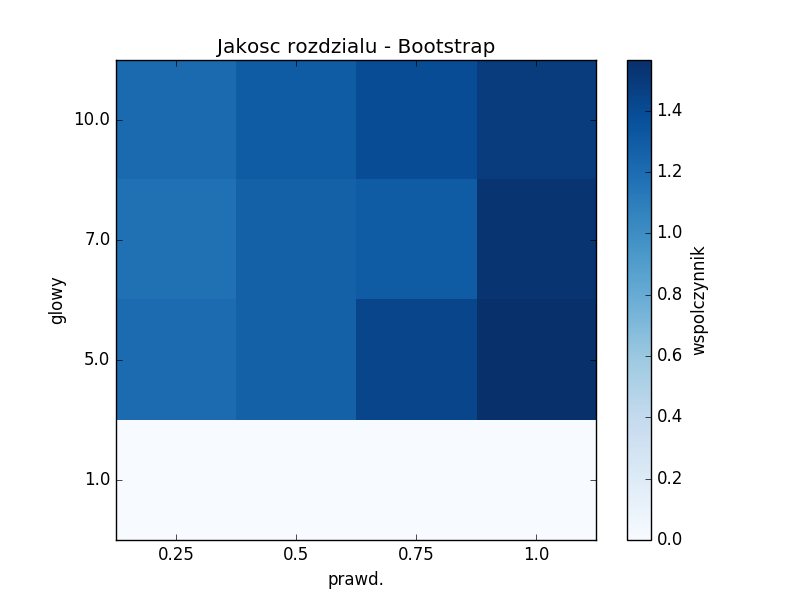
\includegraphics[scale = 0.35]{figures/figures/uncertainties/bootstrap_ratio_mean.png}}{\caption{Bootstrap}\label{fig:b_ratio_mean}}
		\ffigbox{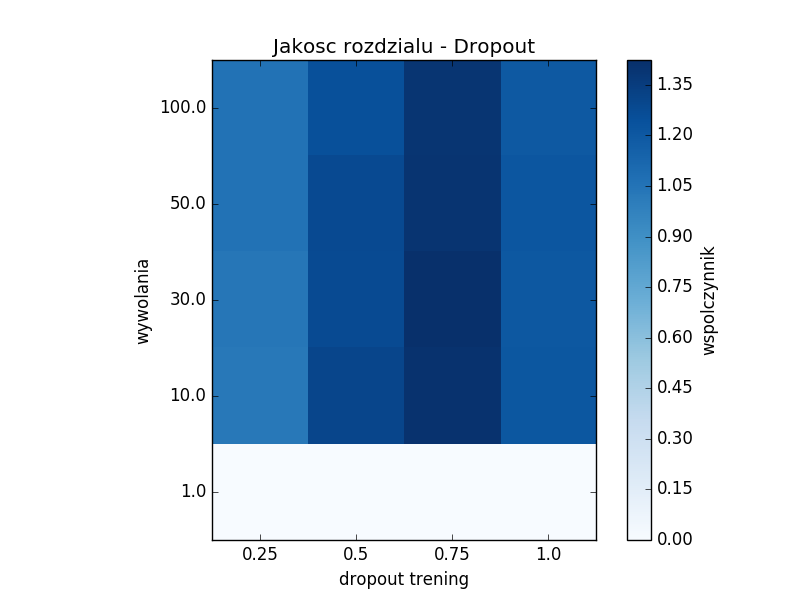
\includegraphics[scale = 0.35]{figures/figures/uncertainties/dropout_ratio_mean.png}}{\caption{Dropout}\label{fig:d_ratio_mean}}
	\end{floatrow}
\end{figure}

\begin{figure}[H]
	\begin{floatrow}
		\ffigbox{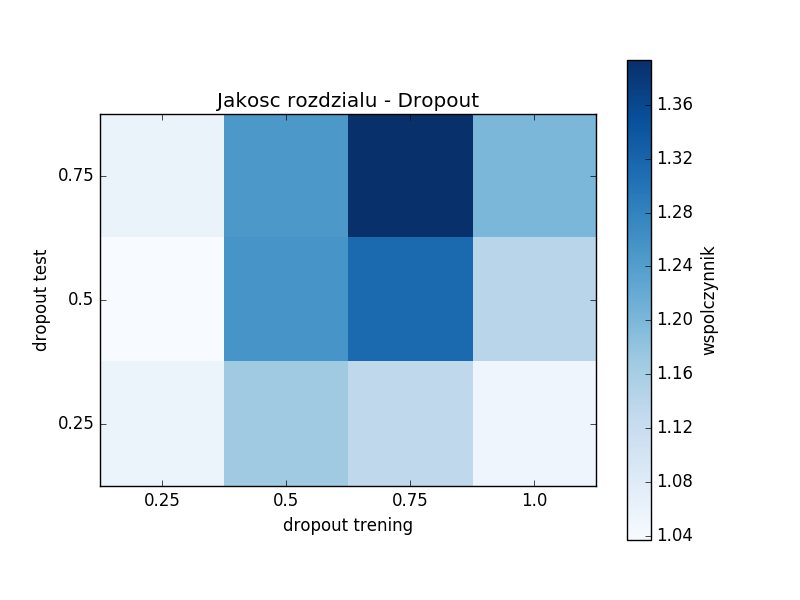
\includegraphics[scale = 0.35]{figures/figures/uncertainties/dropout_ratio_mean2.png}}{\caption{Dropout}\label{fig:d_ratio_mean2}}
		\ffigbox{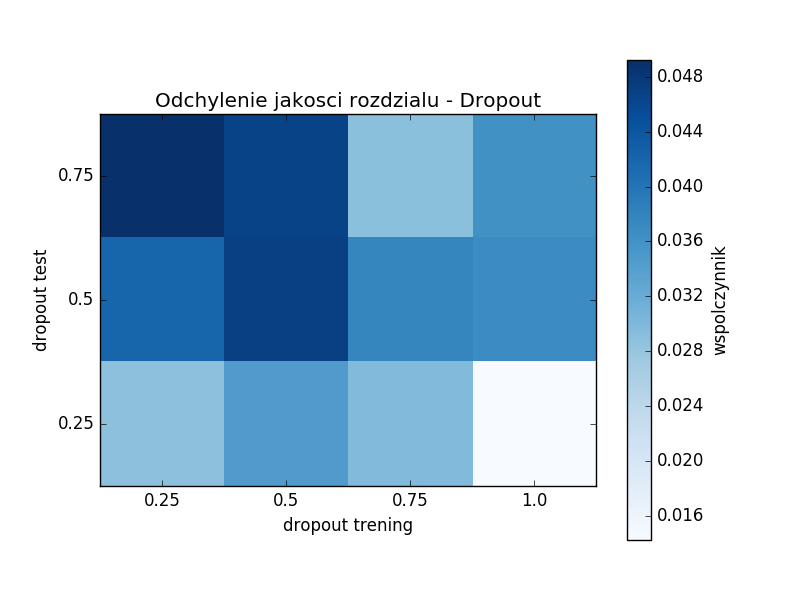
\includegraphics[scale = 0.35]{figures/figures/uncertainties/dropout_ratio_variance2.png}}{\caption{Dropout}\label{fig:d_ratio_var2}}
	\end{floatrow}
\end{figure}

\begin{figure}[H]
	\begin{floatrow}
		\ffigbox{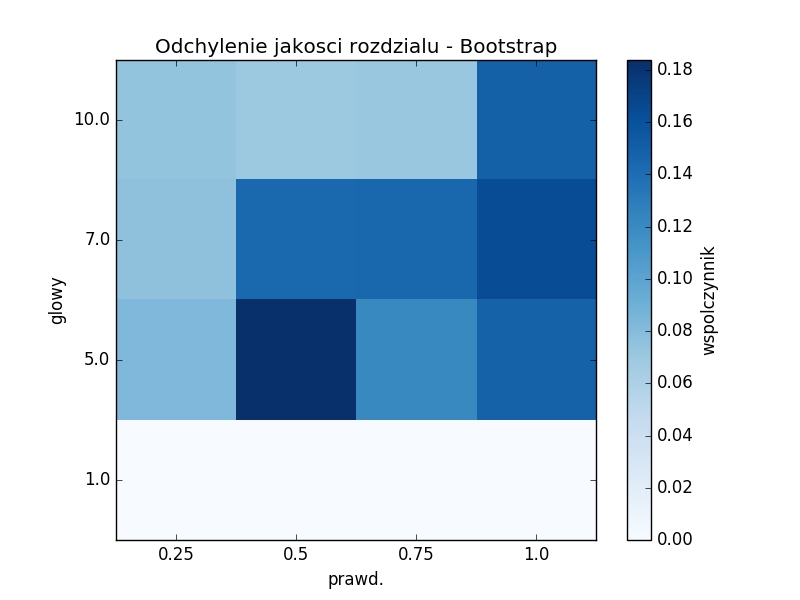
\includegraphics[scale = 0.35]{figures/figures/uncertainties/bootstrap_ratio_variance.png}}{\caption{Bootstrap}\label{fig:b_ratio_var}}
		\ffigbox{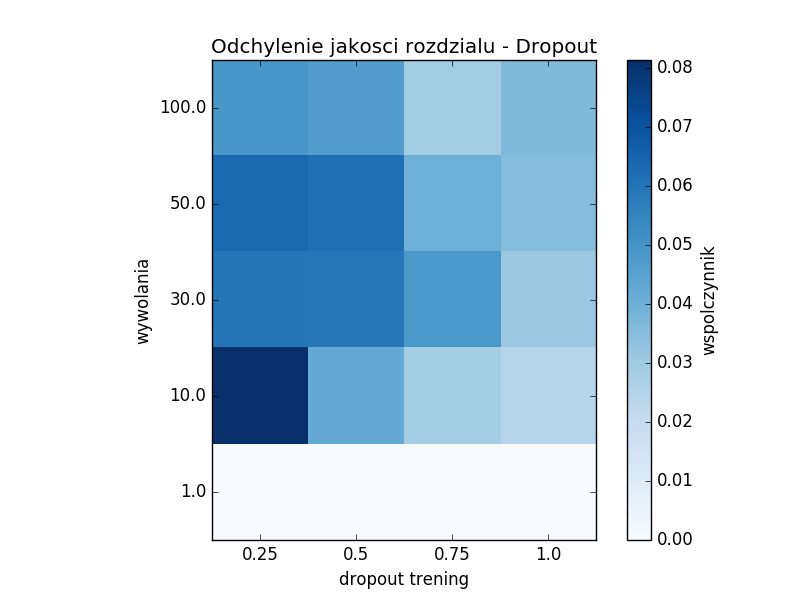
\includegraphics[scale = 0.35]{figures/figures/uncertainties/dropout_ratio_variance.png}}{\caption{Dropout}\label{fig:d_ratio_var}}
	\end{floatrow}
\end{figure}

Na wykresach \ref{fig:b_acc_mean}, \ref{fig:d_acc_mean}, \ref{fig:d_acc_mean2}, \ref{fig:d_acc_var2}, \ref{fig:d_acc_var}, \ref{fig:b_acc_var} przedstawiono średnie i odchylenia standardowe dokładności klasyfikacji uzyskane dla poszczególnych konfiguracji eksperymentów. Wyniki przedstawiają się podobnie jak dla miary $quality_{ND}$. Lepsze wyniki osiąga Bootstrap (44.81\% dla 5 głów i prawdopodobieństwa 0.75, 43.64\%  dla 5 głów i prawdopodobieństwa 1), a jego wyniki są podobne dla wszystkich sensownych parametrów. Wariancja jest minimalna. Wyniki Dropoutu oscylują dookoła 39\% dla wszystkich sensownych parametrów, przy znacznie większej niż Boostrstrap wariancji (2\%). Warto zauważyć, że dla obu metod wyniki są bardzo dodobne dla szerokich zestawów parametrów, i wyraźnie większe niż w przypadku braku bazowego rozwiązania (zaimplementowane w eksperymencie jako Bootstrap z jedną głową, osiągające 37\% dokładności przy 5\% wariancji. Gorszy wynik bazowej wersji wynika z braku odporności na przeuczenie - Bootstrap i Dropout działają jak regularyzatory).


\begin{figure}[H]
	\begin{floatrow}
		\ffigbox{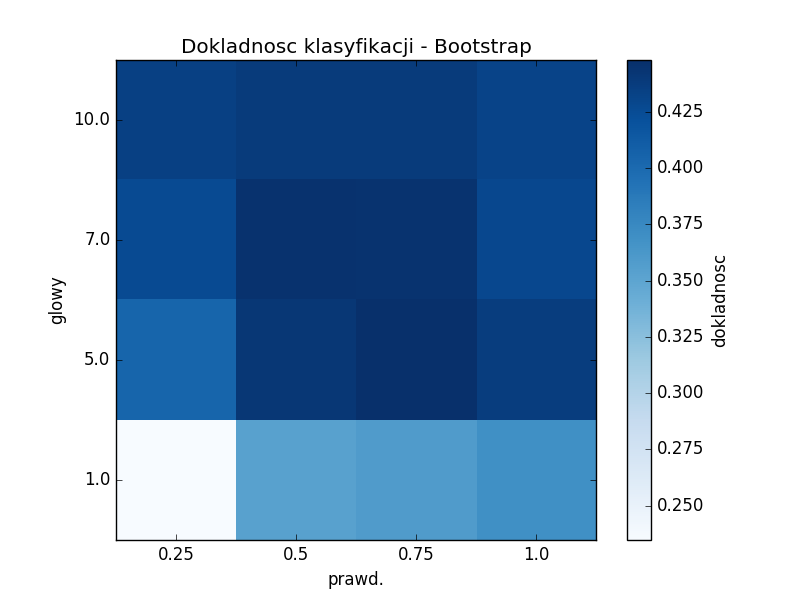
\includegraphics[scale = 0.35]{figures/figures/uncertainties/bootstrap_accuracy_mean.png}}{\caption{Bootstrap}\label{fig:b_acc_mean}}
		\ffigbox{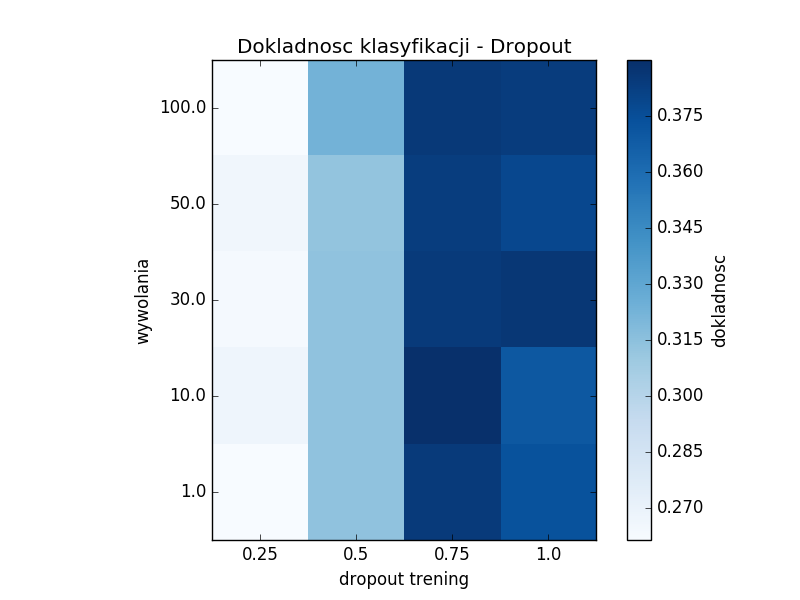
\includegraphics[scale = 0.35]{figures/figures/uncertainties/dropout_accuracy_mean.png}}{\caption{Dropout}\label{fig:d_acc_mean}}
	\end{floatrow}
\end{figure}

\begin{figure}[H]
	\begin{floatrow}
		\ffigbox{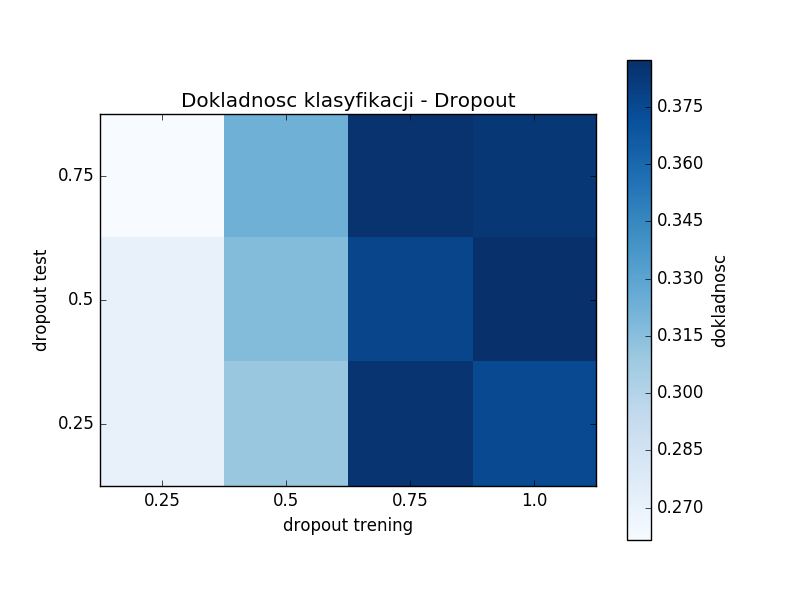
\includegraphics[scale = 0.35]{figures/figures/uncertainties/dropout_accuracy_mean2.png}}{\caption{Dropout}\label{fig:d_acc_mean2}}
		\ffigbox{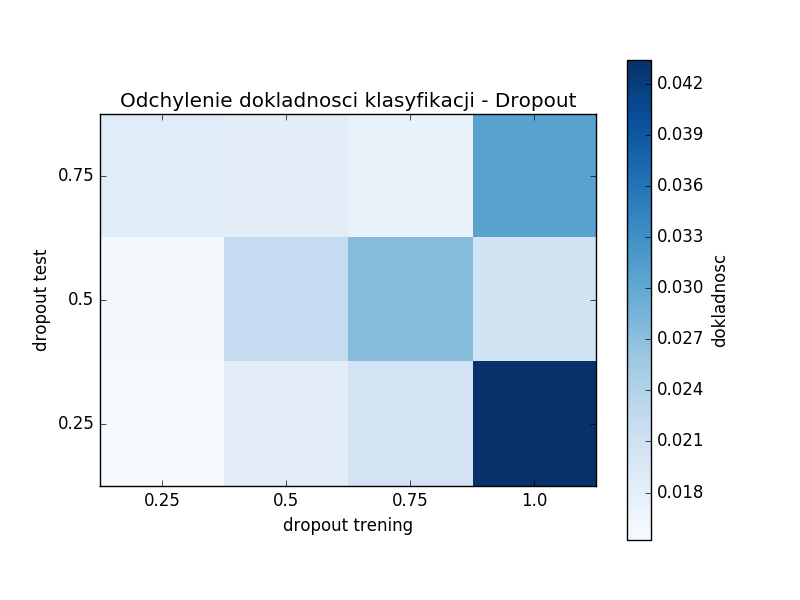
\includegraphics[scale = 0.35]{figures/figures/uncertainties/dropout_accuracy_variance2.png}}{\caption{Dropout}\label{fig:d_acc_var2}}
	\end{floatrow}
\end{figure}

\begin{figure}[H]
	\begin{floatrow}
		\ffigbox{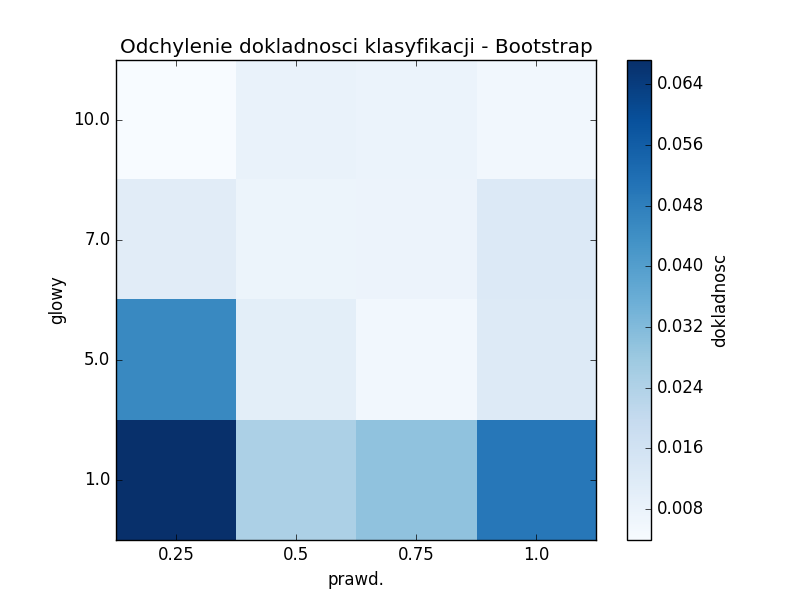
\includegraphics[scale = 0.35]{figures/figures/uncertainties/bootstrap_accuracy_variance.png}}{\caption{Bootstrap}\label{fig:b_acc_var}}
		\ffigbox{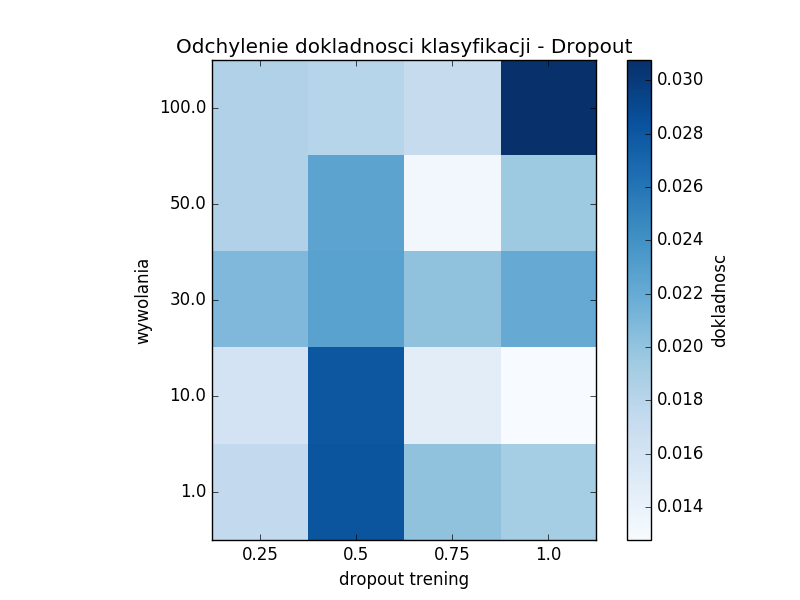
\includegraphics[scale = 0.35]{figures/figures/uncertainties/dropout_accuracy_variance.png}}{\caption{Dropout}\label{fig:d_acc_var}}
	\end{floatrow}
\end{figure}

Na wykresach \ref{fig:b_train_t}, \ref{fig:d_train_t}, \ref{fig:b_test_t}, \ref{fig:d_test_t} przedstawiono czasy treningu i testowania. Na etapie czasu testowania Boostrap wypada znacznie gorzej niż Dropout. 25 sekund dla 5 głów i prawd=0.75 trwa dwa razy dłużej niż 12 sekund osiąganych przez Dropout na wszystkich parametrach, co jest znacznie większym narzutem niż 20\% deklarowane przez autorów metody.

Czas testowania ponownie korzystniejszy jest dla Bootstrapa (0.157s), ponad 5 razy mniej niż Dropout (0.84s). Czas testowania jest bardzo istotny w kontekscie Q-learningu, gdzie dla każdej klatki konieczna jest ocena jakości każdego z możliwych ruchów.

Czas treningu Bootstrapa jest w przybliżeniu liniowo zależny od liczby głów pomnożonych przez prawdopodobieństwo uwzględnienia krotki: $t_{train}  \sim n * p_{incl}$, natomiast czas testu jest w przybliżeniu stały. Czas treningu Dropoutu jest w przybliżeniu stały, natomiast czas testu jest w przybliżeniu liniowo zależny od liczby wywołań $t_{test}  \sim n$.
 
Powody znacznych różnic czasowych mogą tkwić w szczegółach implementacji obu metod. Warto zwrócić uwagę, że dla niektórych zastosowań koszt związany z dodatkowymi obliczeniami może być nieakceptowalny. Natomiast dla zastosowań, dla których koszt działania agenta (czyli koszt zbierania próbek danych) przewyższa koszt działania GPU dłuższy czas działania Bootstrapa może być nieistotny, albo zniwelowany przy wykorzystaniu mocniejszych lub większych zasobów. 

\begin{figure}[H]
	\begin{floatrow}
		\ffigbox{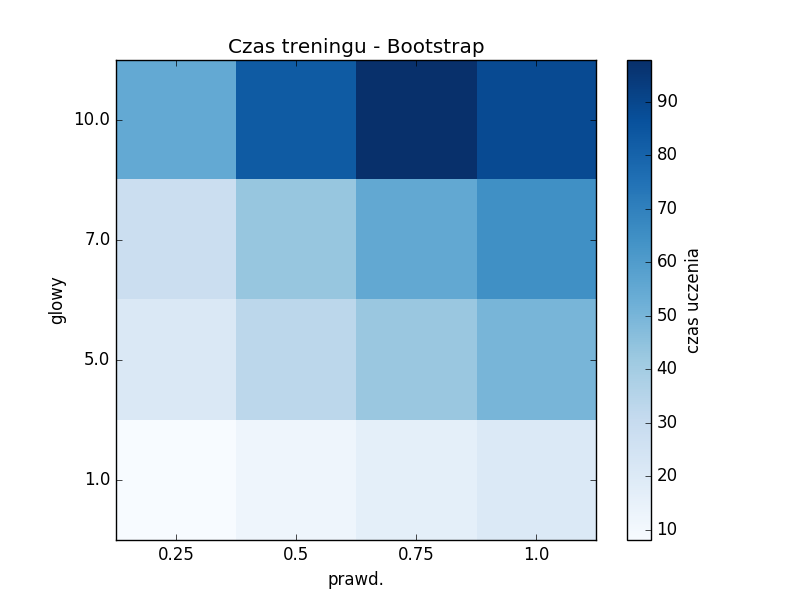
\includegraphics[scale = 0.35]{figures/figures/uncertainties/bootstrap_train_time.png}}{\caption{Dropout}\label{fig:b_train_t}}
		\ffigbox{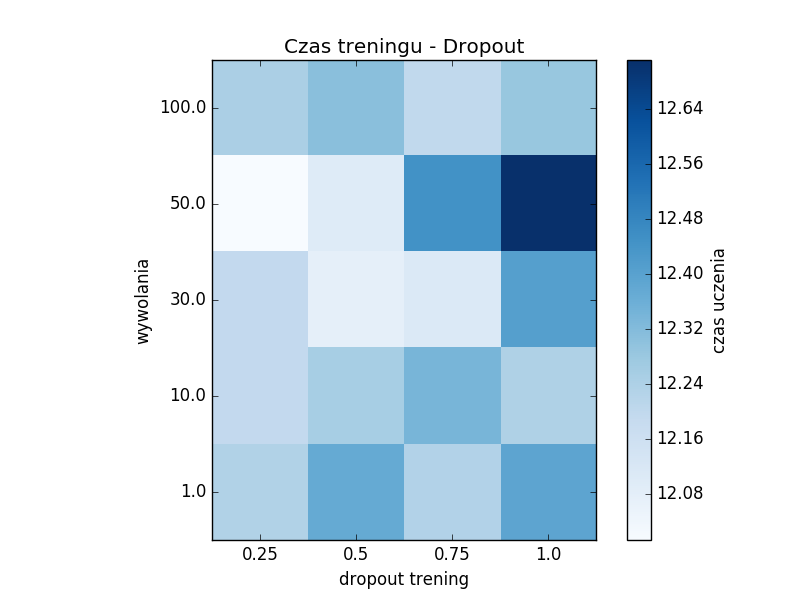
\includegraphics[scale = 0.35]{figures/figures/uncertainties/dropout_train_time.png}}{\caption{Dropout}\label{fig:d_train_t}}
	\end{floatrow}
\end{figure}


\begin{figure}[H]
	\begin{floatrow}
		\ffigbox{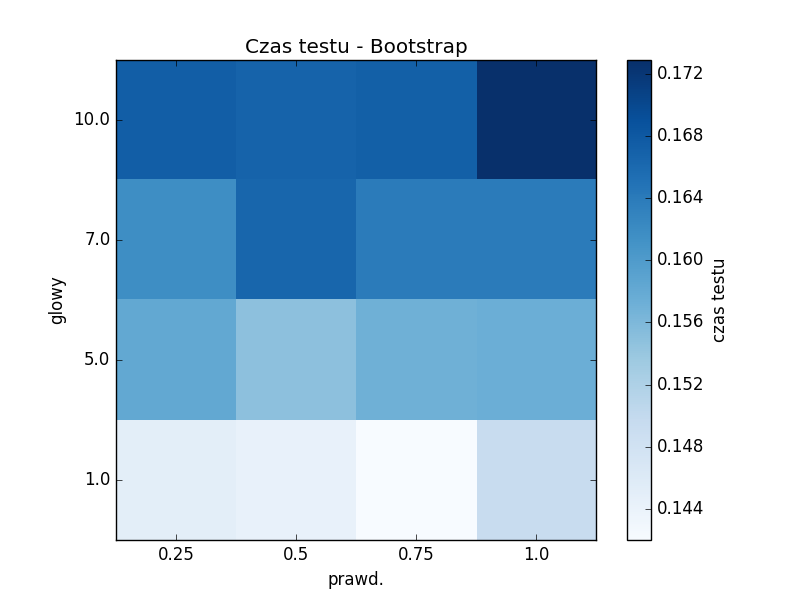
\includegraphics[scale = 0.35]{figures/figures/uncertainties/bootstrap_test_time.png}}{\caption{Dropout}\label{fig:b_test_t}}
		\ffigbox{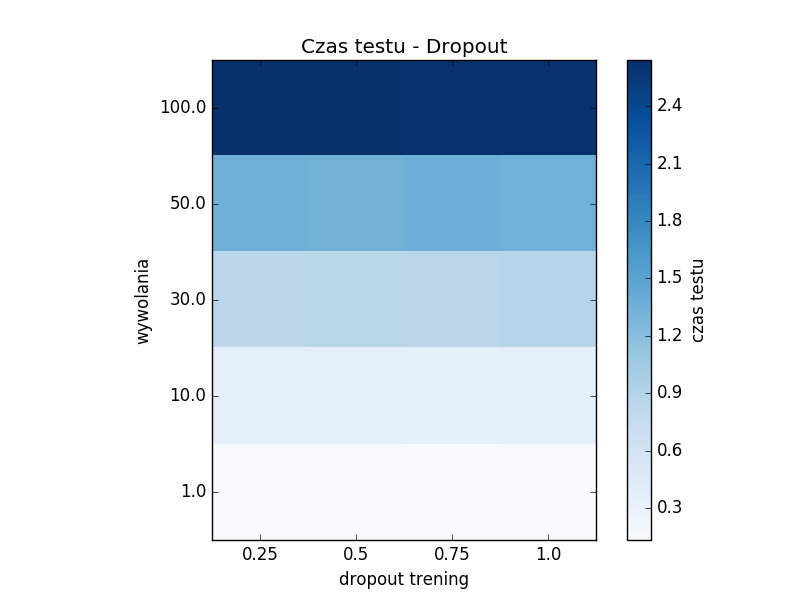
\includegraphics[scale = 0.35]{figures/figures/uncertainties/dropout_test_time.png}}{\caption{Dropout}\label{fig:d_test_t}}
	\end{floatrow}
\end{figure}

Na podstawie przeprowadzonego eksperymentu za najlepszą konfigurację Bootstrapa przyjęto 5 głów i prawdopodobieństwo 0.75, a dla Dropoutu 30 wywołań i oba prawdopodobieństwa równe 0.75

\subsection{Niepewność - wyniki eksperymentu z oceną stopnia pewności}

Dla liczby głów $n=5$ w Bootstrapie i dla liczby wywołań $n=30$ i prawdopodobieństwach dropoutu $p=0.75$ metod współczynnik $quality_{OP}$ dla Bootstrapa z $p=0.75$ wynosi 0.833 przy wariancji 0.11, dla Bootstrapa z $p=1$ wynosi 0.823 przy wariancji 0.10, a dla Dropoutu wynosi 0.925 przy wariancji 0.04. Trafności klasyfikacji dla Bootstrapa z $p=0.75$ wynosi 0.638 a przy wariancji 0.038, dla Bootstrapa z $p=1$ wynosi 0.623 a przy wariancji 0.036 dla Dropoutu wynosi 0.527 przy wariancji 0.032.

\subsection{Niepewność - wnioski}
Bootstrap ma wyraźną przewagę na większości czynników. W drugim eksperymencie jego wyniki są nieznacznie gorsze, ale jako że obie metody osiągają bardzo wysoki współczynnik, ten współczynnik jest pomijalny. Niestety, długi czas treningu Bootstrapa sprawia, że Dropout nie może być kategorycznie odrzucony. Niewykluczone, że w docelowym rozwiązaniu gorsze wyniki Dropoutu będą niezauważalne, natomiast zwiększony czas obliczeń będzie niakceptowalny.

Najważniejszym wnioskiem jest natomiast obserwacja, że obie metody bardzo skutecznie estymują stopień niepewności.


\chapter{Eksperymenty}


% All appendices and extra material, if you have any.
\cleardoublepage\appendix%
%\input{0a-zalacznik.tex}
%\input{0b-pisanie-w-latexu.tex}

% Bibliography (books, articles) starts here.
\bibliographystyle{plalpha}{\raggedright\sloppy\small\bibliography{bibliography}}

% Colophon is a place where you should let others know about copyrights etc.
\ppcolophon

\end{document}
